\documentclass{beamer}
\usepackage[utf8]{inputenc}
\usepackage{graphics}
\usepackage{subcaption}
\mode<presentation> {
\usetheme{unc}}
\setbeamertemplate{navigation symbols}{} % To remove the navigation symbols from the bottom of all slides uncomment this line

\usepackage{graphicx} % Allows including images
\usepackage{booktabs} % Allows the use of \toprule, \midrule and \bottomrule in tables


\usepackage{hyperref}
\hypersetup{linkcolor=blue,colorlinks=true}


% Remove symbols
\beamertemplatenavigationsymbolsempty


%\usetheme{default}

\usefonttheme{serif}

%----------------------------------------------------------------------------------------
%	TITLE PAGE
%----------------------------------------------------------------------------------------


\title[Domestic Politics of Trade]{\LARGE{Domestic Politics and Governance of Trade}}
\author[POLI 150]{Steven Saroka}
\institute{POLI 150}
\date{21 March 2024}


\begin{document}

\begin{frame}
\titlepage % Print the title page as the first slide
\end{frame}


%\begin{frame}
%\frametitle{Overview} % Table of contents slide, comment this block out to remove it
%\tableofcontents % Throughout your presentation, if you choose to use \section{} and \subsection{} commands, these will automatically be printed on this slide as an overview of your presentation
%\end{frame}


%%% SLIDE TEMPLATES

% Template for images
% \begin{frame}{\LARGE Kurdistan}
%     \centering
% \includegraphics[width=\textwidth,height=0.8\textheight,keepaspectratio]{}
% \end{frame}

% %% Core template for the slides
% \begin{frame} 
% \frametitle{\LARGE{}}
% \end{frame}

%----------------------------------------------------------------------------------------
%	PRESENTATION SLIDES
%----------------------------------------------------------------------------------------


% Puzzle framing the class


\begin{frame} 
	\frametitle{\LARGE{Today's Class}}
	\begin{itemize}
		\Large{
			\item Trade and comparative advantage recap 
			\\~\\ 
			\item Why does trade protectionism occur? 
			\\~\\
			\item How do international institutions resolve some trade issues? 
		}
	\end{itemize}
\end{frame}

\begin{frame} 
	\frametitle{\LARGE{Key Terms}}
	\begin{itemize}
		\item Ricardo-Viner Trade Theory
		\item Firm-level trade theory
		\item Domestic influences on trade
		\item Winners and losers from trade
	\end{itemize}
\end{frame}


\begin{frame} 
	\frametitle{\LARGE{Central Question}}
	\centering
	\Large{How do domestic politics impact international trade?}
\end{frame}

\begin{frame}{\LARGE Trade Growth Over Time}
    \centering
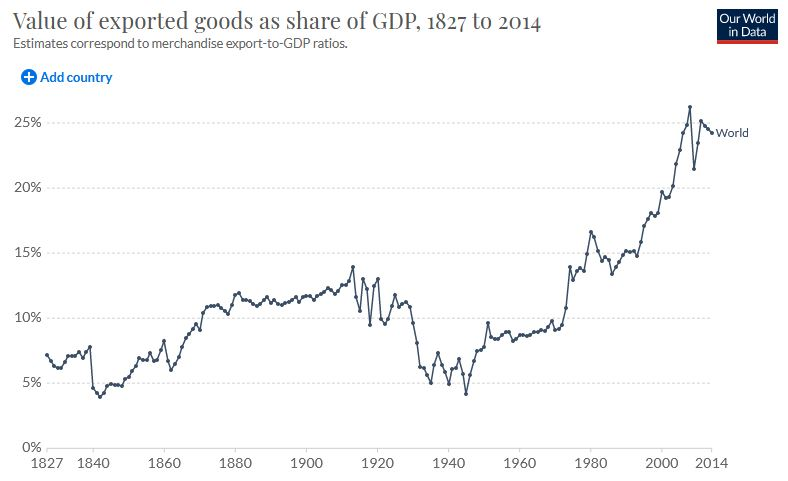
\includegraphics[width=\textwidth,height=0.8\textheight,keepaspectratio]{world export values.JPG}
\end{frame}

\begin{frame}{\LARGE Trade Importance Over Space}
    \centering
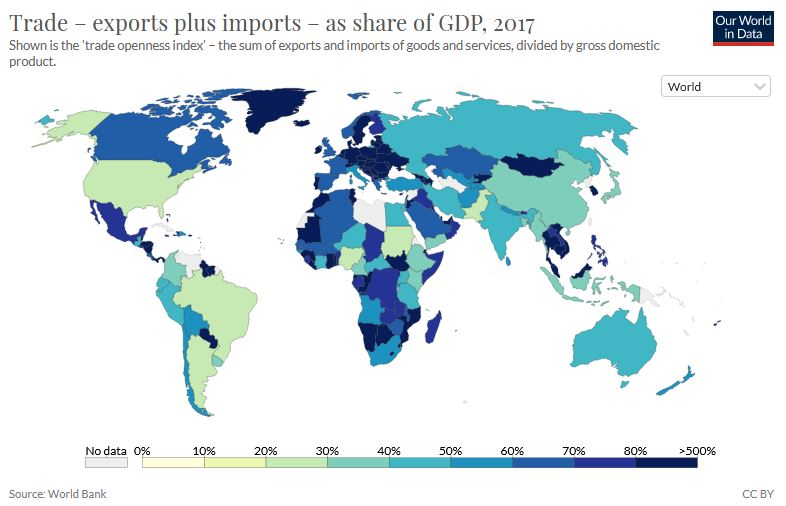
\includegraphics[width=\textwidth,height=0.8\textheight,keepaspectratio]{imports plus exports.JPG}
\end{frame}

\begin{frame} 
	\frametitle{\LARGE Why Trade?}
	\begin{itemize}
			\item (Neo)classical economic and trade theory show that specialization and trade  allow for more production of goods, in an efficient manner. \pause
			\item Different resources allow for \textbf{specialization}.
			\item Thanks to the territorial limits of sovereignty, resources differ by state.
	\end{itemize}
\end{frame}

\begin{frame} 
	\frametitle{\LARGE{Trade and Comparative Advantage}}
	States specialize according to comparative advantage (\textbf{not} absolute advantage). \pause
	\begin{itemize}

			\item \textbf{Absolute advantage}: the ability of a producer to generate a greater number of goods than other producers using the same amount of resources. \pause

			\item \textbf{Comparative advantage}: the ability of a producer to generate a good more efficiently than other goods it could create, so that its most efficient use of resources is to make that specific good/service. \pause 
			\begin{itemize} 
			    \item Can be quantified by \textbf{opportunity cost} of production. \pause
			\end{itemize}
	\end{itemize}
	\textbf{States export those goods for which they have a comparative advantage, and import those for which they do not.}
\end{frame}



\begin{frame}{\LARGE US Exports to Japan}
    \centering
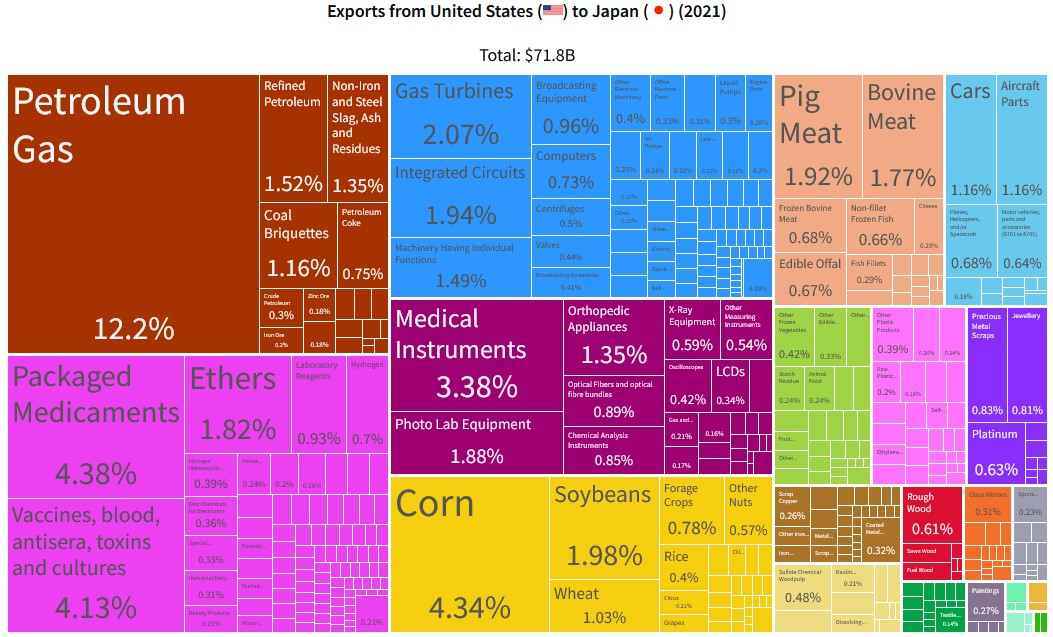
\includegraphics[width=\textwidth,height=0.9\textheight,keepaspectratio]{US to Japan.JPG}
\end{frame}

\begin{frame}{\LARGE Japan Exports to US}
    \centering
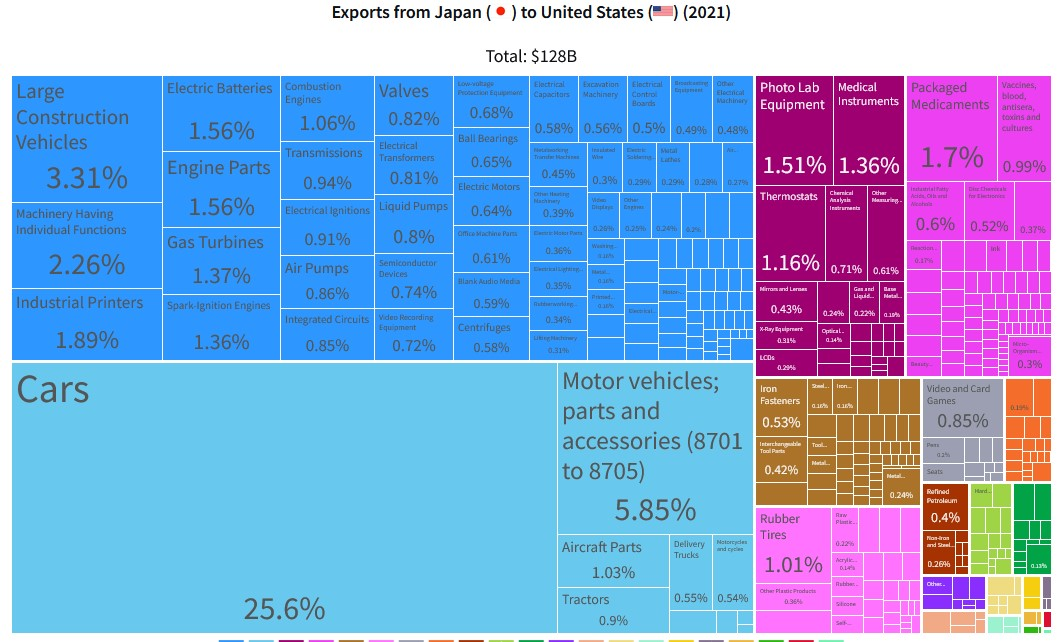
\includegraphics[width=\textwidth,height=0.9\textheight,keepaspectratio]{Japan to US.JPG}
\end{frame}

\begin{frame} 
\frametitle{\LARGE{The Economic Case for Trade}}
Why bother producing and trading according to comparative advantage?
    \begin{itemize}
        \item Larger consumer surplus due to lower world prices (see FLS 342-345). \pause 
        \\~\\
        \item Increasing returns to scale mean more efficient production. \pause 
        \\~\\
        \item Spread of technology. \pause 
        \\~\\ 
        \item Greater economic growth. \pause
    \end{itemize}
\textbf{To summarize the case for free trade according to comparative advantage: more products, more cheaply, in more places while enabling more economic growth.}
\end{frame}

\begin{frame} 
	\frametitle{\LARGE{Sources of Comparative Advantage}}
At the state level, where does comparative advantage come from?
	\begin{itemize}
			\item \textbf{Heckscher-Ohlin trade theory:} comparative advantage comes from an abundance of one or more \textbf{factors of production.} \pause 
			\item \textbf{Ricardo-Viner trade theory:} comparative advantage comes from specific \textbf{sectors/industries}. \pause 
			\item \textbf{Firm-level theory:} comparative advantage comes from size and specialization of important companies.
	\end{itemize}
\end{frame}

\begin{frame} 
	\frametitle{\LARGE{Factors of Production Recap}}
	\begin{itemize}
			\item Land: farming or natural resource extraction. \pause
			\item Labor: generally unskilled labor. \pause
			\item Capital: financial capital and physical capital. \pause
			\item Human capital: skilled labor (sometimes combined with Capital).		
	\end{itemize}
\end{frame}

\begin{frame} 
	\frametitle{\LARGE{Heckscher-Ohlin and ISFM}}
	\begin{itemize}
		\item \textbf{Heckscher-Ohlin trade theory:} states have a comparative advantage when producing goods that make use of whatever factor(s) they have in abundance. \pause 
			\item HO theory assumes \textbf{inter-sectoral factor mobility (ISFM)}: that factors of production can travel easily across economic sectors. \pause
			\item \textbf{Sector:} a component of the economy that produces a specific type of good or service. \pause 
			\begin{itemize}
			    \item Examples: fishing, manufacturing, energy, banking, hospitality, etc. \pause
			\end{itemize}
			\item However, ISFM is really unlikely to be realistic in the short-term... \pause
			\begin{itemize}
			    \item Could physical capital (a factory) used to create cars be used to create pharmaceuticals?
			\end{itemize}		
	\end{itemize}
\end{frame}

\begin{frame} 
	\frametitle{\LARGE{Ricardo-Viner trade theory}}
This criticism of ISFM led to Ricardo-Viner trade theory. \pause
	\begin{itemize}
		\item \textbf{Ricardo-Viner trade theory:} comparative advantage comes not from general factors of production, but from the specific economic sectors in which those factors are located. \pause 
		\item \textbf{How factors are used is more important than the factor itself}. The physical capital used to build cars is not the same as the physical capital used to make pharmaceuticals, even though HO would classify them both as ``capital."
	\end{itemize}
\end{frame}

\begin{frame}{\LARGE US Exports to Japan}
    \centering
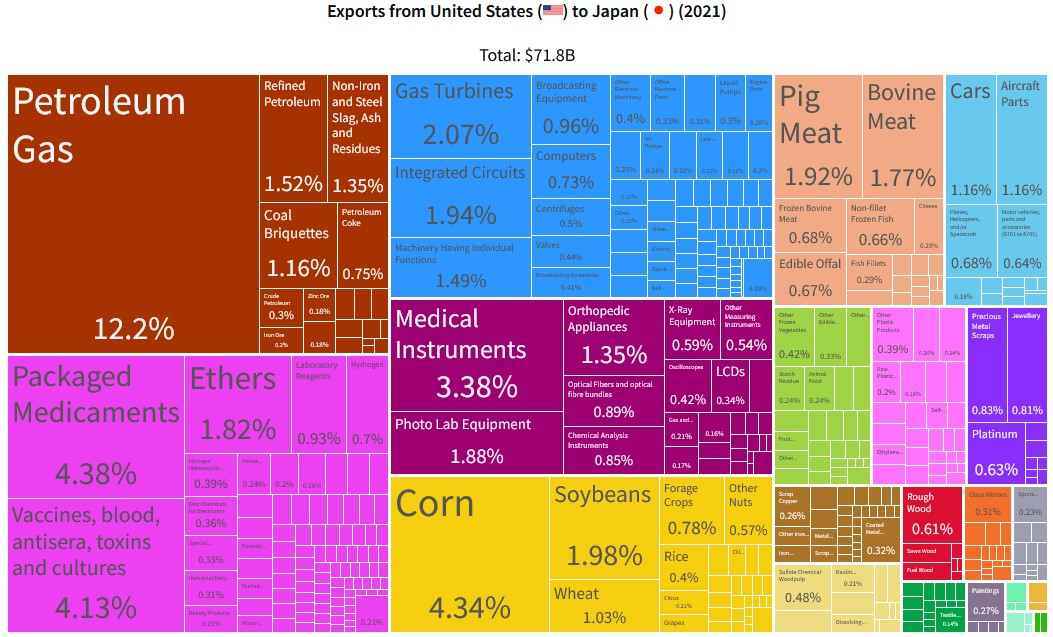
\includegraphics[width=\textwidth,height=0.9\textheight,keepaspectratio]{US to Japan.JPG}
\end{frame}

\begin{frame} 
	\frametitle{\LARGE{Firm-Level Trade Theory}}
	\begin{itemize}
		\item Motivated by the rise of \textbf{multinational corporations} which produce goods in multiple countries. \pause
		\item In practice, international trade is dominated by relatively few MNCs.
		\begin{itemize}
			\item In US, top 1\% of firms account for more than 80\% of exports. \pause
		\end{itemize}
			\item Given this dominance, these ``superstar'' firms may be able to lobby for special political treatment, and may have oversized impact on trade policy considerations. 
	\end{itemize}
\end{frame}

%\begin{frame}{\LARGE Superstar Firms}
 %   \centering
%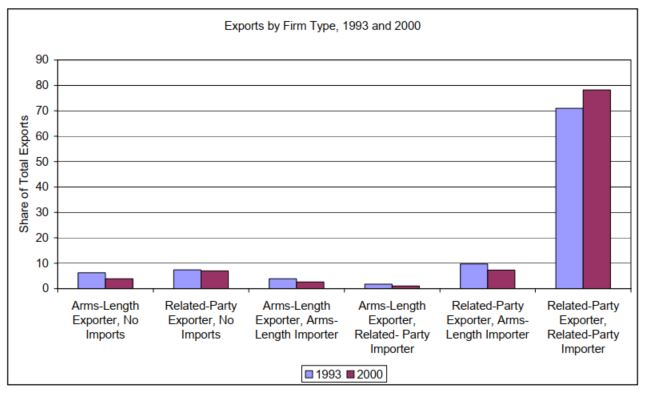
\includegraphics[width=\textwidth,height=0.8\textheight,keepaspectratio]{superstar firms.JPG}
%\end{frame}


\begin{frame} 
	\frametitle{\LARGE{Trade Barriers and Protectionism}}
	\begin{itemize}
		\item Despite a consensus among economists about the economic benefits of free trade, almost every state in the international system engages in \textbf{protectionism}: state-imposed barriers to imports. \pause
		\item Protectionism takes several forms:
		\begin{itemize}
			\item \textbf{Tariffs:} tax on an import, raising the domestic price of that imported good. \href{https://beta.trade.gov/fta/tariff-rates-search}{Explore: ITA's ``What's My Tariff?" tool)} \pause
			\item \textbf{Quotas:} restriction on how much of a foreign good can be imported \href{https://en.vietnamplus.vn/nine-vietnamese-rice-varieties-given-tariff-quotas-in-eu/182888.vnp}{(e.g. Vietnamese rice into the EU)} \pause
			\item \textbf{Non-tariff measures:} rules often related to quality of imports that naturally restrict quantity \href{https://trains.unctad.org/}{(see UNCTAD's online database of NTMs)} 
		\end{itemize}
		\item \textbf{Tariffs are the most common form of protectionism.}
	\end{itemize}
\end{frame}

\begin{frame}{\LARGE Costa Rican Tariffs on Ball Point Pens}
	\centering
	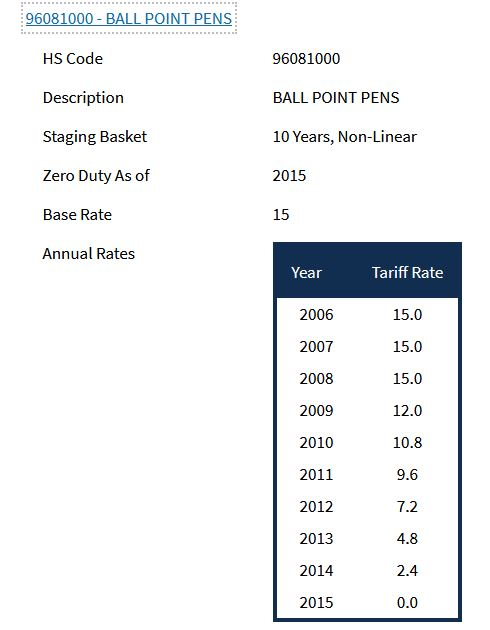
\includegraphics[width=\textwidth,height=0.8\textheight,keepaspectratio]{ball point pens.JPG}
\end{frame}


\begin{frame} 
	\frametitle{\LARGE{Central Question 2}}
	\centering
	\Large{Why do states engage in protectionism?}
\end{frame}


\begin{frame} 
	\frametitle{\LARGE{Puzzle of Protectionism}}
	\begin{itemize}
			\item Protectionism effectively prevents comparative advantage from working to its full effect by altering the balance of imports and exports. \pause
			\item This is counterproductive, from an economic viewpoint. \pause
			\item Additionally, citizens frequently rally \textbf{against} proposed free trade agreements and in favor of protectionist measures.
			\item Example: Trans-Atlantic Trade and Investment Partnership.
	\end{itemize}
\end{frame}

\begin{frame}{\LARGE TTIP Protests}
	\centering
	
\includegraphics[width=\textwidth,height=0.8\textheight,keepaspectratio]{ttip1.jpg}
\end{frame}

%https://www.neweurope.eu/article/thousands-protest-against-ttip-in-berlin/
\begin{frame}{\LARGE TTIP Protests}
	\centering
	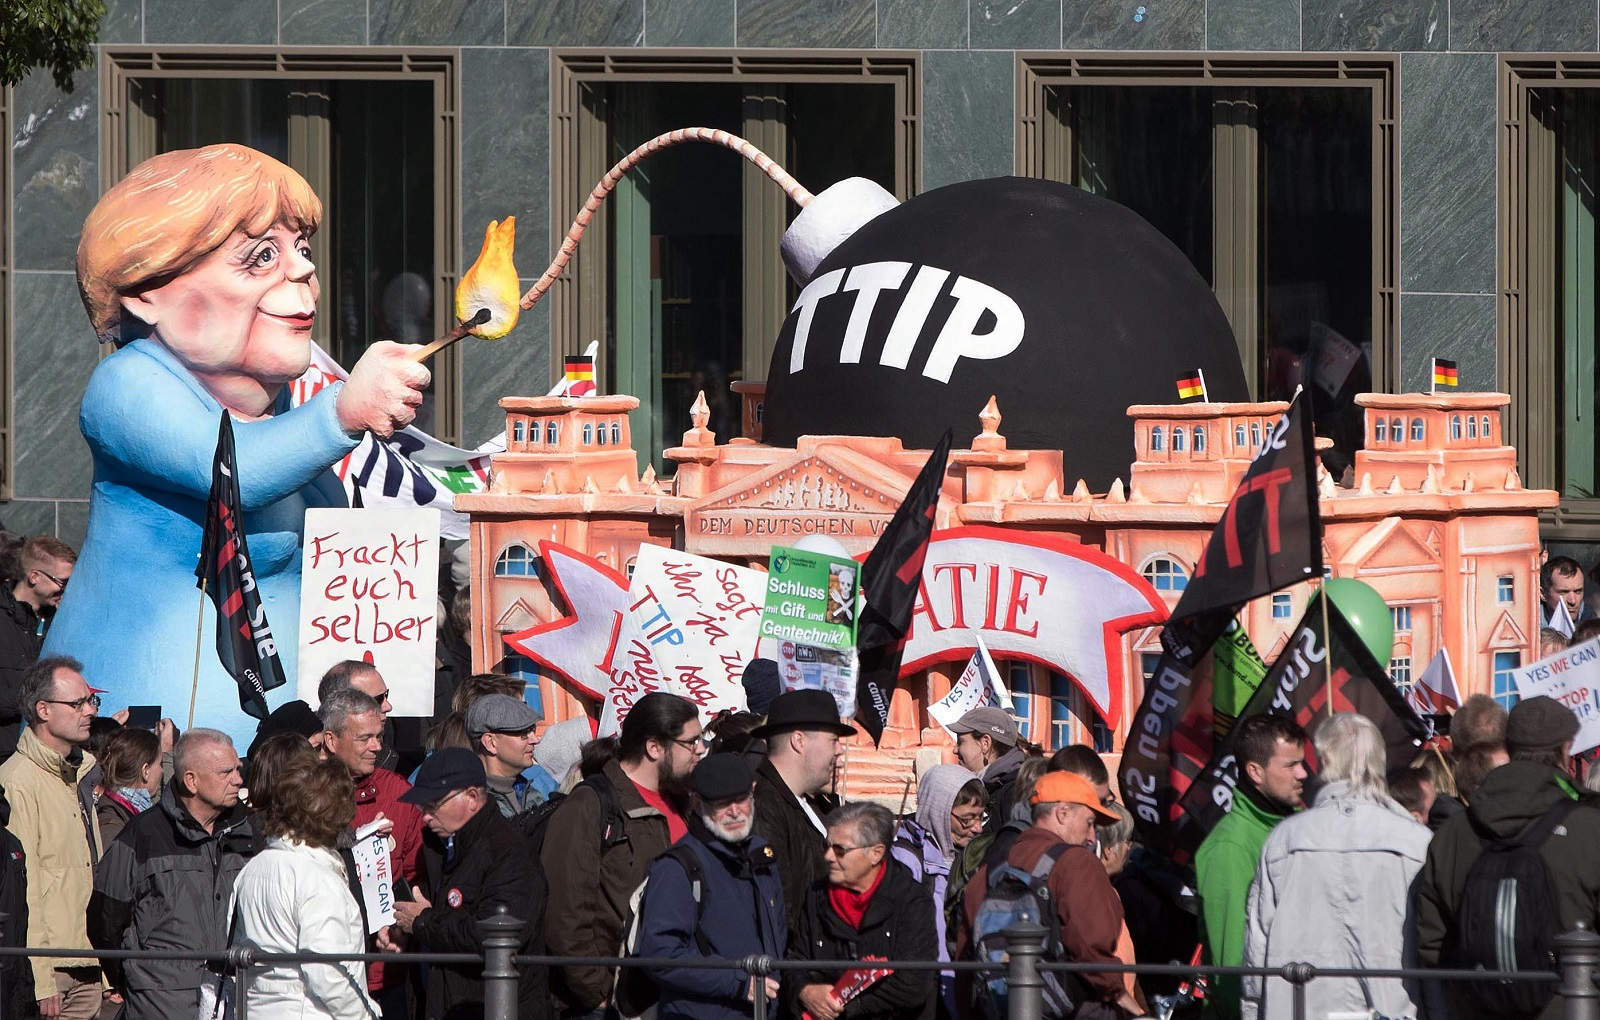
\includegraphics[width=\textwidth,height=0.8\textheight,keepaspectratio]{TTIP-Protests-Berlin.jpg}
\end{frame}

\begin{frame} 
	\frametitle{\LARGE{Domestic Politics of Trade}}
	\begin{itemize}
		\item Why protectionism? \textbf{Because even though trade may boost the economy as a whole, it still has varied distributional effects.} \pause
		\item The economic gains in the aggregate obscure that any trade policy will create winners and losers within any given state. \pause
		\item Thus, the study of the domestic politics of trade is effectively the study of who is hurt or helped by trade in a given state. \pause
		\item So, who are the domestic winners and losers from free trade?
	\end{itemize}
\end{frame}



%\begin{frame}{\LARGE US-China Trade War}
%    \centering
%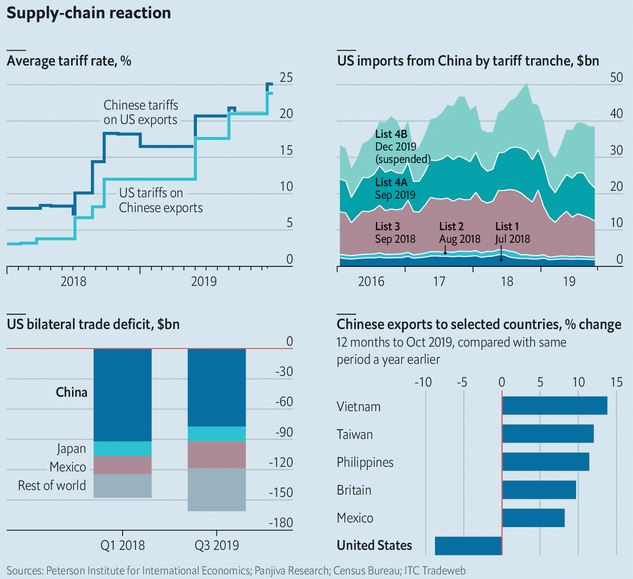
\includegraphics[width=\textwidth,height=0.8\textheight,keepaspectratio]{US-China dispute.JPG}
%\end{frame}




\begin{frame} 
	\frametitle{\LARGE Who Gains From Free Trade?}
	\begin{itemize}
			\item Consumers of imported goods (including as production inputs). \pause 
			\item Exporters (those with a comparative advantage), but which exporters depends on the theoretical approach: \pause 
			\begin{itemize}
				\item Factors/HO theory: trade raises income of relatively abundant factors of production. \pause 
				\item Sectors/RV theory: trade raises income of export-oriented sectors of the economy. \pause 
				\item Firm theory: trade raises income of large firms. \pause 
			\end{itemize}
			\item Citizens in general (FLS example: post-Soviet states), who are often consumers.
	\end{itemize}
\end{frame}

\begin{frame} 
	\frametitle{\LARGE Who Loses From Trade?}
	\begin{itemize}
			\item Producers at a comparative disadvantage who must compete with imports. Again, exact predictions depend on the theoretical approach: \pause 
			\begin{itemize}
				\item Factors/HO theory: Scarce factors of production. \pause 
				\item Sectors/RV theory: Less competitive sectors of the economy. \pause 
				\item Firm theory: Smaller firms. \pause  
			\end{itemize}
			\item \textbf{Each of these groups has a strong interest in trade protection.}
	\end{itemize}
\end{frame}

\begin{frame} 
	\frametitle{\LARGE Gains and Losses by Development Level}
To further complicate things, different factors are winners/losers at different levels of a state's economic development. In the \textbf{Heckscher-Ohlin/factor-based} approach:
	\begin{itemize}
		\item Winners from trade are owners of relatively abundant factor: \pause 
		\begin{itemize}
			\item In rich countries, this is usually high-skill workers/capital.
			\item In poor countries, this is usually (lower-skill) labor. \pause
		\end{itemize}
		\item Losers from trade are owners of relatively scarce factor: \pause 
		\begin{itemize}
			\item In rich countries, this is usually lower-skill labor.
			\item In poor countries, this is usually capital. 
		\end{itemize} 
	\end{itemize}
\end{frame}

\begin{frame} 
	\frametitle{\LARGE Gains and Losses by Development Level}
	The \textbf{Ricardo-Viner/sectoral} approach has a simpler prediction:
	\begin{itemize}
		\item Winners from trade are those employed in sectors that are export industries. \pause 
		\item Losers from trade are those employed in sectors that are import-competing industries.
	\end{itemize}
\end{frame}

\begin{frame} 
	\frametitle{\LARGE Conflict Over Trade}
	\begin{itemize}
			\item Beneficiaries of trade tend to be larger groups (citizen consumers, abundant factors). \pause 
			\begin{itemize}
				\item Like all large groups, they have a collective action problem.
			\end{itemize}
			\item Domestic interaction often occurs between comparatively disadvantaged and comparatively advantaged factors/sectors. 
			\begin{itemize}
				\item Ex: import-competing vs. export-producing industries \pause 
			\end{itemize}
			\item The comparatively disadvantaged are generally fewer in number, while feeling the costs of their disadvantage more acutely than the comparatively advantaged (or general citizen consumers) feel the dispersed benefits of trade.  \pause 
			\item \textbf{Trade protections are thus tend to be narrowly targeted at otherwise uncompetitive factors/sectors that overcome the CAP and lobby for protection.}  
	\end{itemize}
\end{frame}

\begin{frame} 
	\frametitle{\LARGE Trade Conflict and Domestic Institutions}
	\begin{itemize}
		\item Due to their ability to overcome the CAP, comparatively disadvantaged groups should benefit from trade protection fairly often. \pause
		\item However, domestic institutions may impact this, in particular democracy. \pause
		\item If politicians care about voters' wellbeing, they should (in theory) opt for more free trade.
		\item This is especially likely in systems where the chief executive (i.e., president) has a national constituency: if consumers all over the country are harmed by trade protection, and benefit is only enjoyed by small local industry, the president should be more likely to favor free trade...
	\end{itemize}
\end{frame}

\begin{frame}{\LARGE Conflict and Domestic Institutions}
	\centering
	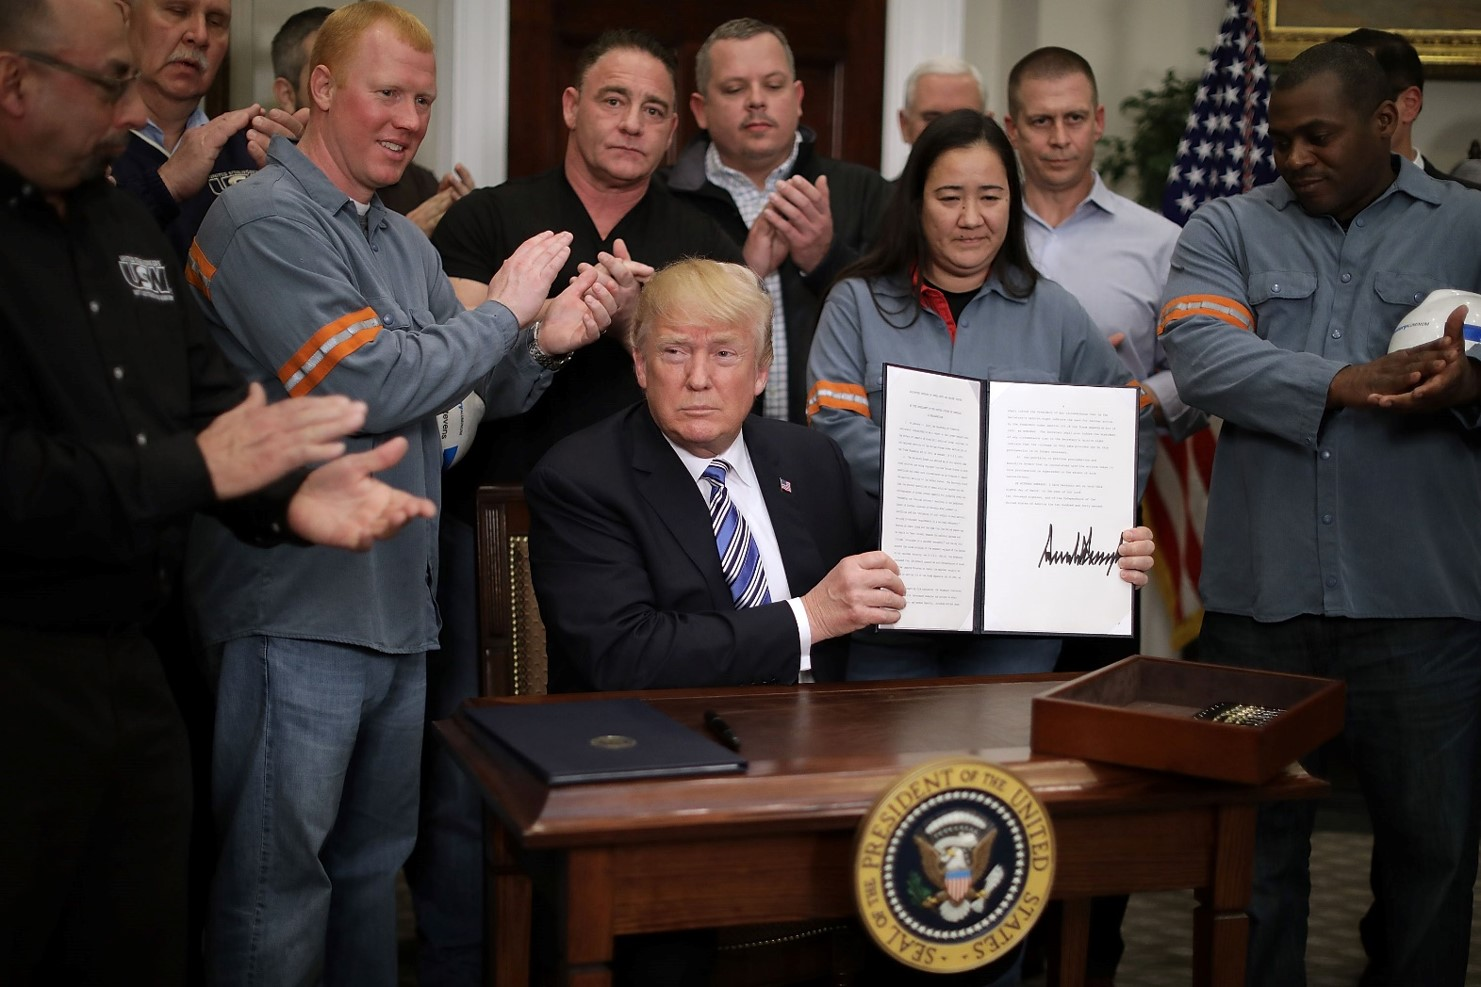
\includegraphics[width=\textwidth,height=0.9\textheight,keepaspectratio]{trump.jpg}
\end{frame}

\begin{frame} 
	\frametitle{\LARGE Trade Protection Winners and Losers}
	\begin{itemize}
		\item The benefit of protectionism is that it protects less-competitive domestic producers from foreign competition, protecting jobs and profits for those producers. \pause
		\item The costs of protectionism come in the form of price increases for protected goods (impacting consumers in general) as well as the state effectively subsidizing businesses that would otherwise fail. 
	\end{itemize}
\end{frame}

\begin{frame}{\LARGE Example: US Sugar Lobby}
	\begin{figure}
		\centering
		\begin{subfigure}{0.49\textwidth}
			\centering
			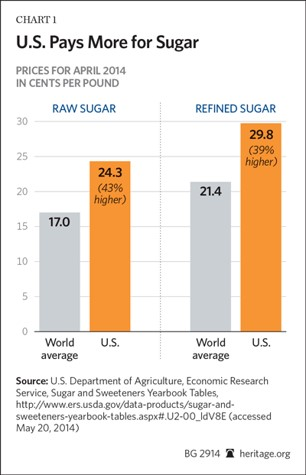
\includegraphics[width = \textwidth,height=.9\textheight]{sugar1.jpg}
		\end{subfigure}
		\begin{subfigure}{0.49\textwidth}
			\centering
			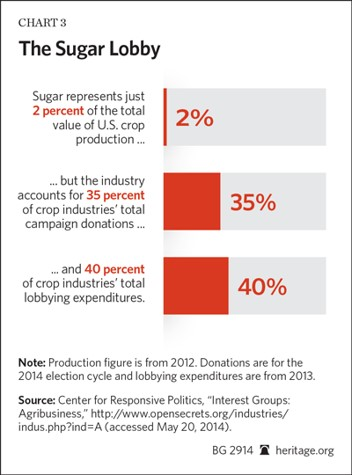
\includegraphics[width = \textwidth, height=.9\textheight]{sugar2.jpg}
		\end{subfigure}
	\end{figure}
\end{frame}

\begin{frame} 
	\frametitle{\LARGE Government Responses}
	\begin{itemize}
			\item Governments can respond to domestic, anti-trade pressures in one of two ways. \pause 
			\item \textbf{Protectionism:} \pause They can institute laws which make it easier for their comparatively disadvantaged interest groups to compete against imports. \pause 
			\begin{itemize}
				\item Subsidies: US to soybeans producers, UAE to Emirates airline. \pause
				\item Tariffs and Quotas: EU on hormone-free beef. \pause 
				\item Non-Tariff Measures: Australian restriction of Canadian salmon on health grounds. \pause 
			\end{itemize}
			\item \textbf{Compensation:} \pause using economic gains from trade to provide trade losers with benefits to offset their losses.
	\end{itemize}
\end{frame}

\begin{frame} 
	\frametitle{\LARGE Compromise of Embedded Liberalism}
	\begin{itemize}
			\item After Great Depression and WWII, US led a coalition of countries to liberalize trade. \pause 
			\item At the same time, these countries expanded their domestic safety nets to help the losers from trade. \pause 
			\begin{itemize}
				\item US: NLRB (1930s), Great Society (1960s) \pause
				\item Sweden: solidarity wages, pension reforms \pause 
			\end{itemize}
		\item This was the \textbf{Compromise of Embedded Liberalism}: sustain popular support for free trade by ensuring that those from less competitive sectors could recover as trade barriers were removed.
	\end{itemize}
\end{frame}

\begin{frame} 
	\frametitle{\LARGE Compromise of Embedded Liberalism}
	\begin{itemize}
		\item The compromise largely ended in the 1970s, especially in US: \pause 
		\begin{itemize}
			\item Tax cuts for corporations \pause 
			\item Scaling back and defunding of social safety nets \pause
			\item Expansion of global finance without similar compensation \pause
		\end{itemize}
		\item Today's Rodrik (2019) article argues that this expansion of globalization without the compromise's safety net (``hyperglobalization") has negative consequences (job losses, financial crises, austerity policies) that have motivated opposition to globalization and economic openness more broadly.
	\end{itemize}
\end{frame}

\begin{frame} 
	\frametitle{\LARGE{Class So Far...}}
	\begin{itemize}
		\large{
			\item Trade produces domestic conflict between winners and losers \pause 
			\\~\\ 
			\item We predict winners and losers using models of comparative advantage \pause  
			\\~\\
			\item Domestic institutions structure those conflicts \pause 
			\\~\\
			\item Governments can respond via protection or compensation, though both have declined over time 
		}
	\end{itemize}
\end{frame}

\begin{frame} 
	\frametitle{\LARGE{Closing Question}}
	\centering
	\Large{What about international financial exchanges?} 
\end{frame}

\end{document}
